\documentclass[12pt]{article}
\usepackage[utf8]{inputenc}
\usepackage{setspace}
\usepackage[textwidth=160mm, textheight=240mm, hmarginratio=1:1, margin=1in]{geometry}
\usepackage{tikz}
\usepackage{tabularx}
\usepackage{graphicx}
\usepackage{titling}
\renewcommand\maketitlehooka{\null\mbox{}\vfill}
\renewcommand\maketitlehookd{\vfill\null}

\title{Determining Pi Lab Report}
\author{Damien Koon}
\date{1/12/23 8:50 CST}

\begin{document}
\maketitle
\doublespacing

\pagebreak

\section{Introduction}

     \hspace{4mm} Over the course of human history, we have long since known about the mathematical constant we now refer to as pi, although many of the ways we have calculated it has changed over time. In the year 250, Archimedes was the first person to accurately measure pi by using a method known as the bisection method. He took a circle and bisected it to make a shape with 12 sides and determined the digits of pi by measuring the perimeter and dividing by the diameter. He repeated this process with more and more sides, eventually stopping at a 96-sided shape, with his approximation of pi being between 3.1429 and 3.1408. (Groleau, 2003) In the 17th century, a mathematician named Ludolph van Ceulen surpassed Archimedes and calculated pi with a circle bisected to have $2^{62}$ sides, which is a little over 4.5 quintillion sides. The work of Ludolph van Ceulen took over 25 years to finish, and the 35 correct decimal places of pi have been inscribed on his tombstone (Lewis 2018). Eventually, Issac Newton devised a new way of calculating pi. When Isaac Newton was 23 and quarantined from the bubonic plague, he made a breakthrough discovery in the binomial theorem $(a + b)^{n} = \sum_{k=0}^{n} \frac{n!}{(n-k!)(k!)} a^{n-k} b^{k}$. He discovered that the binomial theorem works for more than just positive integers as a value for n; he discovered that the binomial theorem also works with negative integers and fractions but creates an infinite series instead of terminating. Newton then had the idea to use the binomial theorem on a circle with the equation $(1-x^{2})^{1/2}$. He then used his newly invented calculus to integrate and calculate the area of a circle using the modified binomial theorem. This led him to find an infinite series that equals pi after some algebraic manipulation. The calculation of pi can now commence with significant precision; before, what took years, now takes a few days of arithmetic (Ye, 2016) 

\pagebreak

        We determined the famous mathematical constant, pi, analytically and graphically in our experiment. We used measuring tools, such as string, rulers, and meter sticks, to surmise the lengths of the diameter and circumference of five separate circular objects. The diameter of a circle is the length directly across the circle, and the circumference is the length around the circle's perimeter. Once we had compiled all of our measured values, we began to estimate pi analytically. To determine pi, with a degree of uncertainty, we divided the circumference by the diameter to approximate pi. In some of our measurements of the circular objects, we had introduced a lot of uncertainty implicit in measuring objects that are not perfectly circular., while others had less. For example, larger objects with rougher edges were not perfectly circular. They thus had a higher level of uncertainty, and smaller objects were difficult to get accurate measurements with because of the smaller distance used with the ruler. . To account for this change in uncertainty from object to object; we estimated pi using five different objects. We then averaged our results together to achieve an average value of pi at 3.09 with a percentage error of 1.64\%. After analytically estimating pi, we used our estimated value of the circumference and diameter to plot points on a graph. When we took the slope of this graph, we had a graphical representation of pi.

\pagebreak

\section{Part 1: Determination of Pi - Calculation Method}

    \hspace{6mm}\textbf{Objectives:}
    \\ \hspace{4mm} Exploring measurements and forms of error \\
    
    \textbf{Types of Error:}
    \\ \hspace{4mm} Random errors: These types of errors have no pattern and can be seen \\ in fluctuations in your results between each trial. These types of errors cannot be predicted or avoided.
    \\ \hspace{4mm} Systematic Errors: These types of errors can result from issues with equipment and instruments. These errors occur on a consistent basis each time a measurement is taken. Examples include uncalibrated balances, faulty instruments due to wear and tear, or consistently misusing an instrument by fault of the person. \\

    \textbf{Materials required:}
    \\ \hspace{4mm} 5 small, circular household items
    \\ \hspace{4mm}String: should be long enough to wrap around the largest circular item you use!
    \\ \hspace{4mm} Ruler
    \\ \hspace{4mm} Calculator
    \\ \hspace{4mm} Graph paper \\



    \textbf{Procedure:}
    \\ 1. \hspace{2mm} Write a description of the circular object you measure in Column 1 in the cart. (i.e., "coffee cup," "peanut butter lid," canned soup," etc.)
    \\ 2. \hspace{2mm} Using a ruler, measure the diameter in centimeters to 3 sig figs for each object. The diameter is the straight line passing from side to side in the center of a circle. (If the diameter stops directly on a marking on the ruler i.e., 3 cm, your value should be recorded as 3.00 cm. If it stops at, i.e., 2.5 cm, your value should be recorded as 2.50 cm.) Record the value for diameter in column 2 in the chart.  
    \\ 3. \hspace{2mm} Take the string and wrap it around the circular object - the length of the string will represent the circumference of the circle
    \\ 4. \hspace{2mm} Line the string up against the ruler to correctly measure the circle's circumference in centimeters to 3 significant figures. Record the value of circumference in Column 3 in the chart.
    \\ 5. \hspace{2mm} Divide the object's circumference by diameter. Record the value in Column 4 in the chart. This value should be very close to the value for Pi. Note that Pi has no units. Your value in Column 4 should be in 3 sig figs.
    \\ 6. \hspace{2mm} Take the average of your values for Column 4 and record the value for "Average" under the chart. \\

    
\begin{tabularx}{.8\textwidth} { 
  | >{\centering\arraybackslash}X 
  | >{\centering\arraybackslash}X 
  | >{\centering\arraybackslash}X 
  | >{\centering\arraybackslash}X | }

 \hline
 Description of Disk & Diameter (cm) & Circumference (cm) & Circumference divided by Diameter \\
 \hline
 Blue Diamond \textbf{Bold} Almonds Container  & 8.48 cm  & 26.5 cm & 3.13  \\
\hline
 Blue Diamond \textbf{Bold} Almonds lid  & 8.65 cm  & 27.8 cm & 3.21  \\
\hline
 Hand sanitizer  & 14.5 cm  & 40.8 cm & 2.81  \\
\hline
 Battery & 3.25 cm & 10.6 cm & 3.26  \\
\hline
 Protractor  & 8.91 cm  & 27.3 cm & 3.06  \\
\hline
 
\end{tabularx}

\pagebreak

\section{Sample Calculations}

\hspace{5mm} I measured the lid of a container of Blue Diamond \textbf{BOLD} Almonds with Wasabi \& Soy Sauce flavoring. I measured the diameter to be 8.65cm and the circumference to be 27.8cm. Using the two values, I determined pi to be 3.21.
$$\frac{Circumference}{Diameter} = \frac{27.8cm}{8.65cm} = 3.21$$

For the graphical method, I used two points separate from my original points on the graph. The two points I used were (4cm, 12cm) and (6cm, 18cm). Using the point-slope formula, I determined pi to be 3.00. 
$$slope = m = \frac{18cm-12cm}{6cm - 4cm} = \frac{6cm}{2cm} = 3.00$$

1. \hspace{2mm} The accepted value for pi is 3.1516. Calculate the percentage error of your average value for pi. Under 10\% is a realistic goal. Do you consider your value for pi to be close to the accepted value? Express your answer in 3 significant figures. $$Percentage Error = \frac{|3.1416-average|}{3.1416}*100\ = \frac{|3.1416-3.09|}{3.1416} * 100\% = 1.64\% $$

2. \hspace{2mm} What are some potential benefits and drawbacks of determining the value for pi using this method? List one benefit and one drawback. 
\\ \indent It is inaccurate because of the uncertainty implicit in measurement. It is beneficial to have repeated trials to decrease errors and approach the correct value, pi.

3. \hspace{2mm} We made several measurements for the value of pi using this method. Why do you think we need to make more than one measurement?
\\ \indent When you take measurements of a large set of data, you will get a regression to the mean effect, which appears as a bell curve on a graph. When you take the average of a more extensive data set, you will get a more accurate approximation. 

\pagebreak

\section{Part II: Determination of pi - Graphical method}

\hspace{4mm}On a separate sheet of graph paper, plot points using the circumference and diameters of each object from Part I where the (x,y) = diameter, circumference). You must draw your graph by hand - do not use a computer program to make your graph. Make the y-axis "circumference (cm)" and the x-axis "Diameter (cm)." Use the following steps to create your graph: \\

\noindent 1. Draw the x-axis and the y-axis using a ruler \\
\\ \noindent 2. Label your graph using the instructions above \\
\\ \noindent 3. Make a scale to fit your graph (you may use different scales for each axis) \\
\\ \noindent 4. Plot your points on the graph \\
\\ \noindent 5. Draw a line of best fit through your points on the graph, making sure to start from the origin; this is a straight line through the points, beginning at the origin. Do NOT connect the dots, but draw a straight line with a ruler that passes through or near the dots. You may have points just above or below the line of best fit. \\
\\ \noindent 6. Pick 2 points on the line you drew (not including an of your original points) and find the x-location and y-location of each. Record the values on the next page. \\
$$x_1 location: 4cm$$
$$y_1 location:12cm$$
$$x_2 location: 6cm$$
$$y_2 location: 18cm$$

\noindent 7. Find the slope of the line. \\
$$Slope = \frac{y_2-y_1}{x_2-x_1}$$
$$m = \frac{18cm-12cm}{6cm-4cm} = \frac{6cm}{2cm} = 3cm$$ 

\noindent 8. Did you get the same as the average value for pi in Part I? \\
\indent No, $3 \not= 3.09$ 

\noindent 9. What are some potential benefits and drawbacks of determining the value for pi using this graphical method? List one benefit and one drawback.

Drawing the line of best fit introduces error, and so does the scale at which you draw your graph. Drawing the graph with the slope showing a graphical representation of the mathematical constant. 

\noindent 10. List at least two forms of error you encountered while determining the value for pi in parts I and II - two from part I and two from part II. Categorize the errors as random and/or systematic.

A form of error in measurement would be introduced by using objects that are not perfectly circular. There is also a form of error introduced by our puny human eyes when using rulers and string for measurement. The non-circular objects introduced systematic errors in our measurements as well. In the graphical method, errors were introduced by hand drawing the line of best fit on the graph and using a scale that could have had more detail to assist in accuracy. \\
\pagebreak

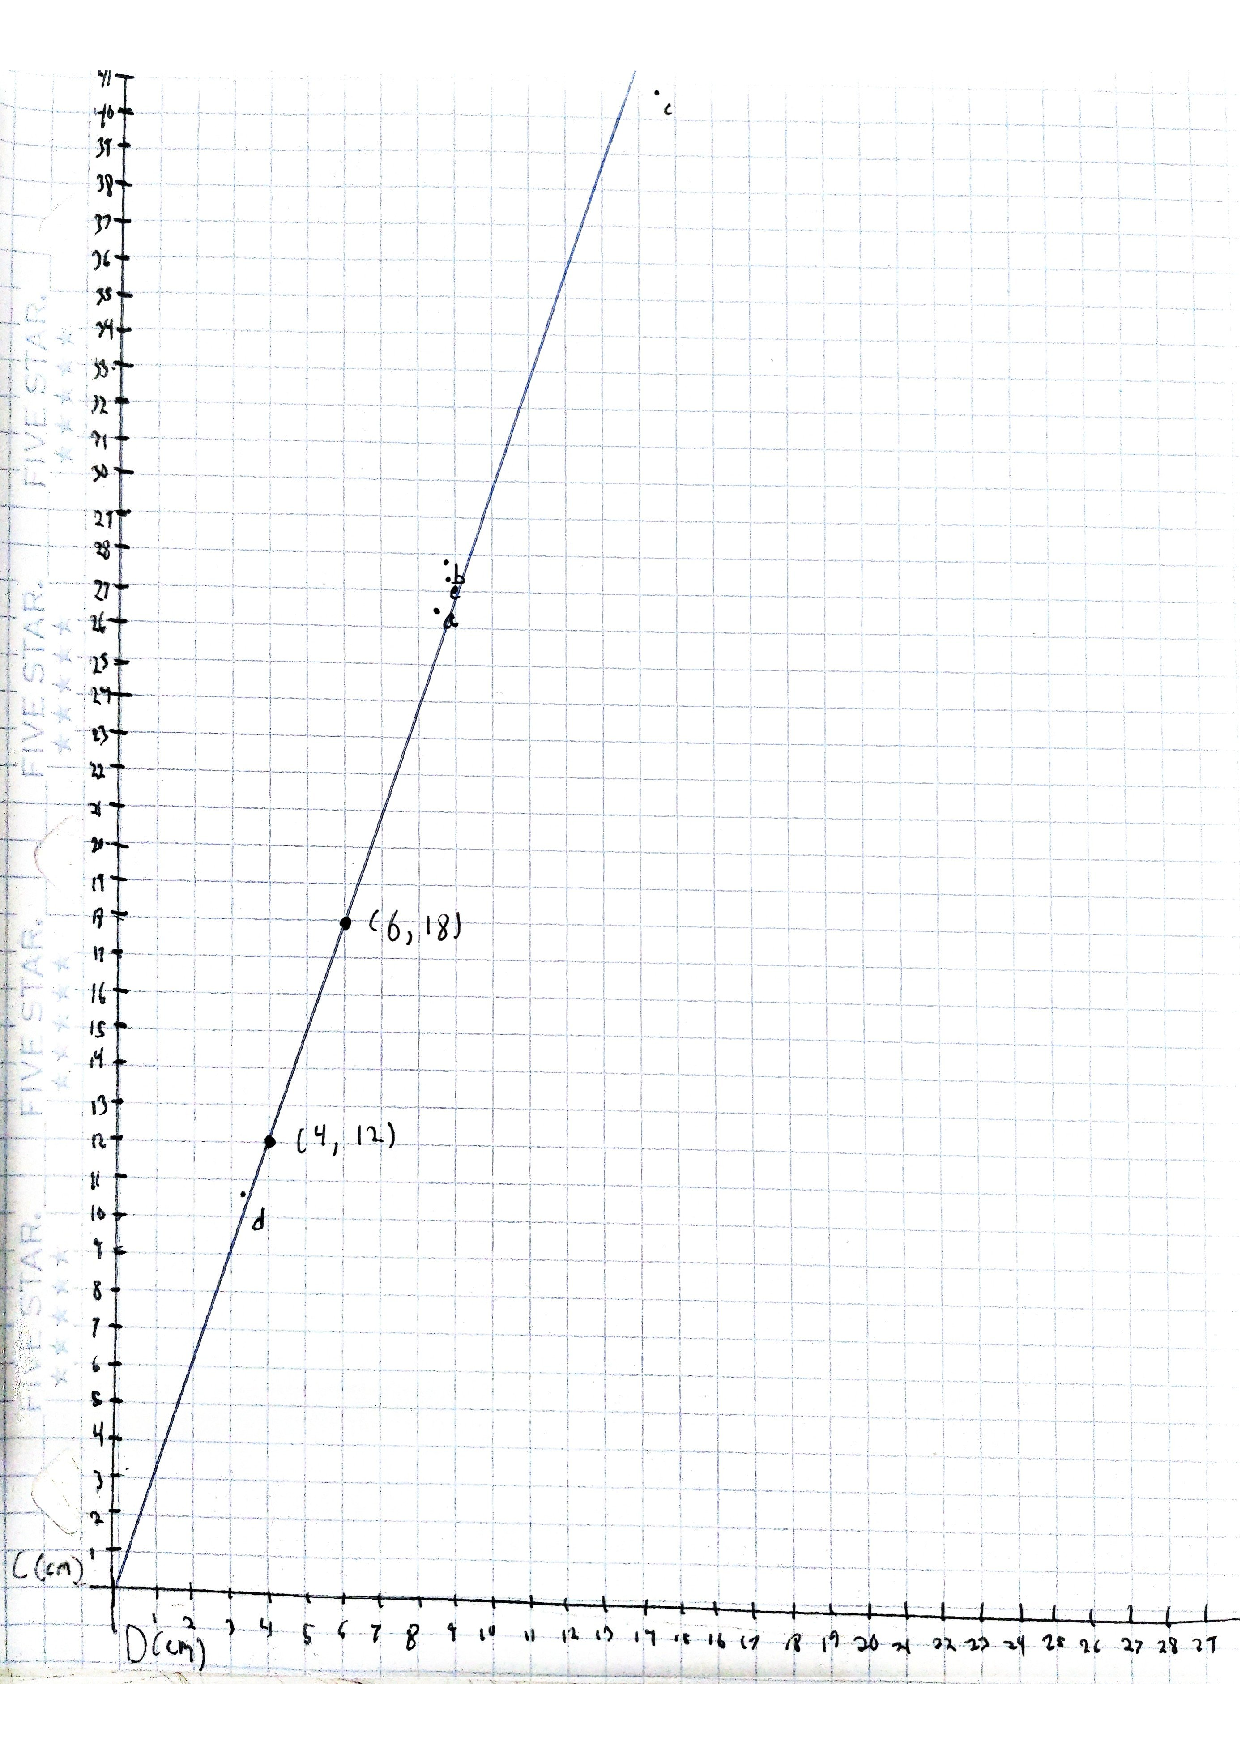
\includegraphics[scale=0.8]{PiReportGraph}

\pagebreak

\section{Conclusion}

\hspace{4mm} In the determining pi lab, we estimated pi to be 3.09. This value is only 0.05 off the expected value, with an error of 1.64\%. We had more uncertainty with certain objects in the analytical trials than others. For example, using a large container of hand sanitizer was the farthest from pi because it was rounded towards the bottom. We also had a lot of uncertainty in measuring the battery; this is because the battery was very small at only 3.25cm in diameter. This smaller size made it more difficult to be accurate with the ruler when measuring. After we finished the analytical method of measuring and calculating pi, we moved on to a different approach of graphically representing pi and determining the value with the point-slope formula. For the graphical method, we made a graph with the circumference as the Y-axis and the diameter as the X-axis. We plotted all 5 points we measured previously on the graph and then made a line of best fit. Two separate points were marked on the graph, and then the slope was calculated using the point-slope formula. Using the graphical method, our estimated value was 3.00. Using the measurement and analytical method, there was more accuracy at the cost of random error. There was less accuracy in the graphical method, but it had a visual correspondence of pi to go along with it. The slope of the line in the graphical method gave a different value of pi because of the scale of my graph as well as the error that is introduced from drawing the line of best fit. If I had changed my scales to increase precision, I would have more accurate estimates of pi. Many forms of error were introduced, some were systematic, and some were random. In our calculations, the only systematic errors were from using the graphical method. Using the analytical method only introduced errors randomly through measurement. \\ \\

\pagebreak

\textbf{References:} \\
Groleau Rick (2003) Approximating Pi \\
https://www.pbs.org/wgbh/nova/physics/approximating-pi.html \\

\noindent Ye Xiaojing (2016) The Long Search for the Value of Pi \\
https://www.scientificamerican.com/article/the-long-search-for-the-value-of-pi/ \\

\noindent Lewis Hazel (2018) Celebrating Pi Day – Ludolph van Ceulen, another forgotten hero of Pi \\
https://www.mathscareers.org.uk/celebrating-pi-day-ludolph-van-ceulen/ \\



    
    
    

\end{document}
